\documentclass{lehramt-informatik-haupt}
\usepackage{amsmath}
\usepackage{blkarray}
\usepackage{tikz}
\usetikzlibrary{arrows.meta}

\begin{document}

%-----------------------------------------------------------------------
%
%-----------------------------------------------------------------------

\section{AB 6: Aufgabe 5 (Check-Up)}

Ein gerichteter Distanzgraph sei durch seine Adjazenzmatrix gegeben (in
einer Zeile stehen die Längen der von dem Zeilenkopf ausgehenden Wege.)
\footcite[Seite 3]{aud:ab:6}

\[
\begin{blockarray}{cccccc}
& M & A & P & R & N \\
\begin{block}{c(ccccc)}
  M & - & 5 & 10& - & - \\
  A & - & - & 3 & 9 & 2 \\
  P & - & 2 & - & 1 & - \\
  R & - & - & - & - & 4 \\
  N & 7 & - & - & 6 & - \\
\end{block}
\end{blockarray}
\]

\begin{enumerate}

%%
% (a)
%%

\item Stellen Sie den Graph in der üblichen Form dar.

\paragraph{Lösung gezeichnet mit \href{https://www.ctan.org/pkg/pgf}{TikZ}}

\begin{center}
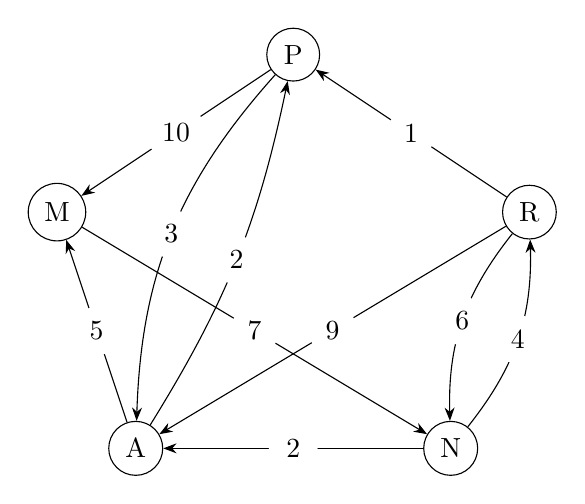
\begin{tikzpicture}
\begin{scope}[every node/.style={circle,draw}]
  \node (M) at (-1,0) {M};
  \node (A) at (0,-3) {A};
  \node (P) at (2,2) {P};
  \node (R) at (5,0) {R};
  \node (N) at (4,-3) {N};
\end{scope}

\begin{scope}[>={Stealth[black]},
              every node/.style={fill=white,circle},
              every edge/.style={draw=black}]
  \path [->] (A) edge node {$5$} (M);
  \path [->] (P) edge node {$10$} (M);
  \path [->, bend angle=20, bend right] (P) edge node {$3$}  (A);
  \path [->] (R) edge node {$9$} (A);
  \path [->] (N) edge node {$2$} (A);
  \path [->, bend angle=10, bend right] (A) edge node {$2$} (P);
  \path [->] (R) edge node {$1$} (P);
  \path [->, bend angle=20, bend right] (N) edge node {$4$} (R);
  \path [->] (M) edge node {$7$} (N);
  \path [->, bend angle=20, bend right] (R) edge node {$6$} (N);
\end{scope}
\end{tikzpicture}
\end{center}

\paragraph{Lösung gezeichnet online auf
\href{http://graphonline.ru/en/?graph=uhkywkYEzLukCUxf}{graphonline.ru}}

\par

\url{http://graphonline.ru/en/?graph=uhkywkYEzLukCUxf}

\begin{center}
\includegraphics[width=0.6\linewidth]{Aufgabe-5_Check-Up_graphonline.ru.png}
\end{center}

%%
% (b)
%%

\item Bestimmen Sie mit dem Algorithmus von Dijkstra ausgehend von $M$
die kürzeste Wege zu allen anderen Knoten.

\paragraph{Nach der Methode von
\href
{https://www.youtube.com/watch?v=4pBP2hbnGso}
{Prof. Dr. Oliver Lazar}}

\begin{tabular}{|l|l|l|l|l|l|}
\hline
Schritt & Betrachteter Knoten & Kosten A & Kosten P & Kosten R & Kosten N \\\hline
Initial & M                   &          &          &          & 7        \\\hline
1       & N                   & 9        &          & 11       & 7        \\\hline
2       & A                   & 9        & 11       & 11       & 7        \\\hline
3       & P                   & 9        & 11       & 11       & 7        \\\hline
4       & R                   & 9        & 11       & 11       & 7        \\\hline
\end{tabular}

\paragraph{Nach der Methode aus der Vorlesung}

\textbf{Besuchte Knoten:} M

\begin{tabular}{l||l|l|l|l|l}
Knoten-Name & M    & A        & P        & R        & N \\\hline
Distanz     & 0    & $\infty$ & $\infty$ & $\infty$ & $\infty$ \\
Vorgänger   & null & null     & null     & null     & null \\
\end{tabular}

\textbf{Besuchte Knoten:} M, N

\begin{tabular}{l||l|l|l|l|l}
Knoten-Name & M    & A        & P        & R        & N \\\hline
Distanz     & 0    & $\infty$ & $\infty$ & $\infty$ & 7 \\
Vorgänger   & null & null     & null     & null     & M \\
\end{tabular}

\textbf{Besuchte Knoten:} M, N, A

\begin{tabular}{l||l|l|l|l|l}
Knoten-Name & M    & A        & P        & R        & N \\\hline
Distanz     & 0    & 9        & $\infty$ & $\infty$ & 7 \\
Vorgänger   & null & N        & null     & null     & M \\
\end{tabular}

\textbf{Besuchte Knoten:} M, N, A, P

\begin{tabular}{l||l|l|l|l|l}
Knoten-Name & M    & A        & P        & R        & N \\\hline
Distanz     & 0    & 9        & 11       & $\infty$ & 7 \\
Vorgänger   & null & N        & A        & null     & M \\
\end{tabular}

\textbf{Besuchte Knoten:} M, N, A, P, R

\begin{tabular}{l||l|l|l|l|l}
Knoten-Name & M    & A        & P        & R        & N \\\hline
Distanz     & 0    & 9        & 11       & 11       & 7 \\
Vorgänger   & null & N        & A        & N        & M \\
\end{tabular}

\paragraph{Ergebnis}

$M \rightarrow N = 7$

$M \rightarrow N \rightarrow A = 9$

$M \rightarrow N \rightarrow A \rightarrow P = 11$

$M \rightarrow N \rightarrow R = 11$

%%
% (c)
%%

\item Beschreiben Sie wie ein Heap als Prioritätswarteschlange in diesem
Algorithmus verwendet werden kann.

\begin{antwort}
Die Prioritätswarteschlange kann dazu verwendet werden, den Knoten mit
der kürzesten Distanz schnell zu finden. Eine Prioritätswarteschlange
kann zum Beispiel durch eine Min-Heap realisiert werden. Wenn eine
Min-Heap aufgebaut wird, ist das Minium immer das Wurzelelement. Es kann
sehr einfach und schnell entnommen werden. Der Aufbau einer Min-Heap
geht mit linearem Zeitaufwand $\mathcal{O}(n)$ vonstatten. Die
Entnahme des Miniums schlägt im schlechtesten Fall mit einem Aufwand
von $\mathcal{O}(\log n)$ zu Buche schlagen.
\end{antwort}

%%
% (d)
%%

\item Geben Sie die Operation \emph{„Entfernen des Minimums“} für einen
Heap an. Dazu gehört selbstverständlich die Restrukturierung des Heaps.

\begin{antwort}
Bei der Entnahme des Minimums wird an dessen Stelle das am Ende
der Halde sich befindende Element gesetzt.

Das neue Minimum verletzt unter Umständen die Heap-Eigenschaften, wenn
eines oder beide seiner Kind-Knoten kleiner sind. Es muss mit dem
kleinsten Kind-Knoten getauscht werden. Diese Prozedur wird rekursiv so
lange ausgeführt, bis die Heap-Eigenschaften wieder hergestellt sind.
Man nennt diesen Vorgang auch \texttt{heapify}.

Es kann aber auch sein das das verschobene Element kleiner ist. Dann
muss die gegenteilige Operation von \texttt{heapify} ausführt werden,
die \texttt{decrease} genannt wird.
\end{antwort}

\end{enumerate}

\end{document}
